% [Borrador pase 2. Fusión de ch5_resultados.tex + ch6_discusion.tex en un único capítulo
% "Resultados y Discusión" (estructura híbrida: resultado + su interpretación en el mismo lugar).
% Datos: matrix_prod_v1 (wiki/datos/matrix_prod_v1.md; data/runs/matrix_prod_v1/
% {analisis,sensibilidad_*}.json). Figuras: chapters/images/ch5/. Destino: chapters/ch5_resultados_discusion.tex]

\chapter{Resultados y Discusión}
\label{ch:Results}

Este capítulo presenta los hallazgos del estudio comparativo y los interpreta. El orden
es el del razonamiento empírico. Primero se confirma que el simulador reproduce las
referencias analíticas, para que las diferencias posteriores puedan atribuirse al método
y no a un artefacto del modelo. Se recuerda a continuación el diseño del contraste y las
métricas que se reportan, y se caracteriza la forma del paisaje de optimización que cada
régimen de bloqueo de modos presenta a la búsqueda, clave que ordena la lectura de lo que
sigue. Sobre esa base se exponen e interpretan, tema por tema, el desempeño comparado y
su contraste estadístico, el comportamiento del sustituto neuronal, la forma física de
las soluciones y su robustez local. El capítulo cierra con una síntesis que responde a la
pregunta de investigación y reconoce los límites de validez del estudio. Todo enunciado
cuantitativo se ancla en una figura, una tabla o una prueba; la matriz de datos que lo
respalda está documentada en el conjunto \texttt{matrix\_prod\_v1}.

\section{Validación del modelo numérico}
\label{sec:res_validacion}

Antes de comparar los algoritmos se verifica que el entorno de evaluación reproduce
las soluciones analíticas conocidas. El procedimiento completo (con sus pruebas de
convergencia) se desarrolló en la Sección~\ref{sec:sim_verificacion}; esta sección
recoge la evidencia gráfica que respalda esa validación, porque de ella depende que
las diferencias entre métodos puedan atribuirse a la búsqueda y no al simulador.

La comprobación de partida contrasta el perfil estacionario del simulador con las
soluciones cerradas del marco teórico. La Figura~\ref{fig:res_val_perfiles} superpone,
para los tres casos canónicos, la intensidad $|A|^2$ obtenida numéricamente y su forma
analítica: la gaussiana de Kuizenga--Siegman del régimen activo (ecuación~\eqref{eq:tau_gauss}; duración $\tau_p=91.4$~ps), la secante hiperbólica del absorbente rápido en el régimen pasivo (ecuación~\eqref{eq:tau_pasivo}; $52.3$~ps) y el solitón activo de Kärtner (Sección~\ref{sec:ml_activo_soliton}; $21.6$~ps). En los tres, los puntos
analíticos caen sobre la curva numérica sin desviación apreciable; el acuerdo en
duración es del orden del $0.01\%$ para el caso de Kuizenga--Siegman y de la fracción
del uno por ciento para el solitón.

\begin{figure}[htbp]
  \centering
  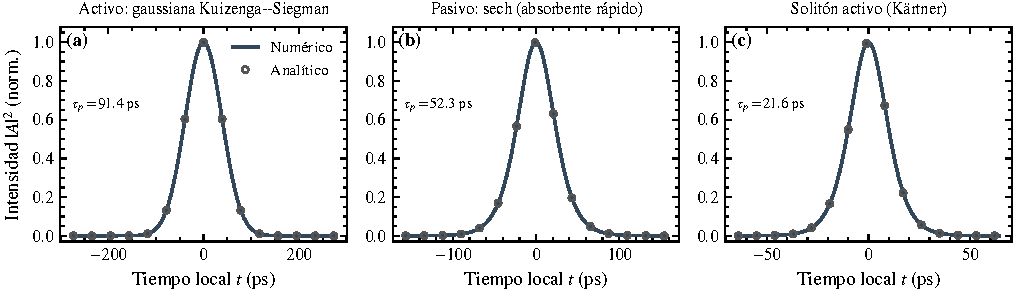
\includegraphics[width=\textwidth]{chapters/images/ch5/fig_val_perfiles.pdf}
  \caption[Validación del perfil estacionario del pulso]{Validación del perfil estacionario: intensidad $|A|^2$ normalizada,
  numérica (línea) frente a analítica (círculos), en los tres casos canónicos: gaussiana de Kuizenga--Siegman (activo), secante hiperbólica del absorbente rápido
  (pasivo) y solitón activo de Kärtner. Los puntos analíticos se solapan con la curva
  numérica en los tres casos.}
  \label{fig:res_val_perfiles}
\end{figure}

Reproducir la forma final no basta: interesa además que el simulador alcance el
atractor correcto por la dinámica de la cavidad y no por imposición. La
Figura~\ref{fig:res_val_transitorio} sigue la duración y la energía del pulso a lo
largo de las vueltas para la formación de un solitón. Partiendo de una semilla ancha,
la duración atraviesa un transitorio con el batido característico entre el solitón y el continuo (Sección~\ref{sec:ml_activo_soliton}; oscila y se ensancha hacia las primeras centenas de vueltas) antes de
relajarse, hacia las dos mil vueltas, al valor analítico ($\approx 24$~ps); la energía
crece en paralelo y satura cerca de $40$~nJ. El criterio de estado estacionario
adoptado detiene la integración una vez extinguido ese transitorio, de modo que los
observables se miden sobre el atractor y no sobre un estado intermedio.

\begin{figure}[htbp]
  \centering
  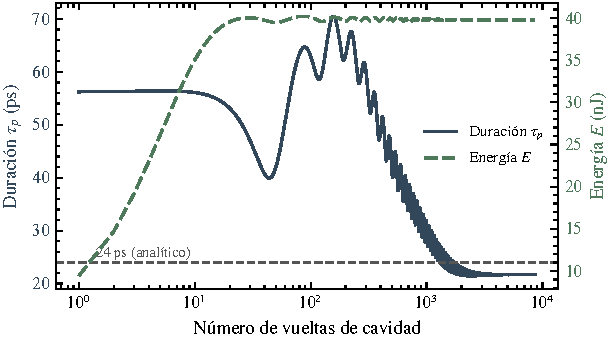
\includegraphics[width=0.7\textwidth]{chapters/images/ch5/fig_val_transitorio.pdf}
  \caption[Transitorio de formación del pulso]{Transitorio de formación del pulso: duración $\tau_p$ (izquierda) y energía
  $E$ (derecha) frente al número de vueltas de cavidad (eje logarítmico). Tras el
  batido solitón--continuo de las primeras centenas de vueltas, la duración se relaja
  al valor analítico ($24$~ps, línea discontinua) y la energía satura cerca de
  $40$~nJ.}
  \label{fig:res_val_transitorio}
\end{figure}

La validación se extiende del punto a la región que los optimizadores van a explorar.
La Figura~\ref{fig:res_val_mapa_regimenes} clasifica el estado estacionario sobre el
plano de parámetros de cada régimen, ganancia y profundidad de modulación
$(g_0, M)$ en el activo, ganancia y pérdida no saturada $(g_0, q_0)$ en el pasivo,
distinguiendo monopulso, extinción y falta de convergencia. En ambos regímenes el
monopulso ocupa la mayor parte del dominio; la extinción y la no convergencia se
confinan a franjas estrechas cerca de las fronteras (modulación muy baja en el activo,
ganancia insuficiente frente a la pérdida en el pasivo). El espacio de búsqueda es, por
tanto, mayoritariamente factible, con las regiones penalizadas acotadas a sus bordes.

\begin{figure}[htbp]
  \centering
  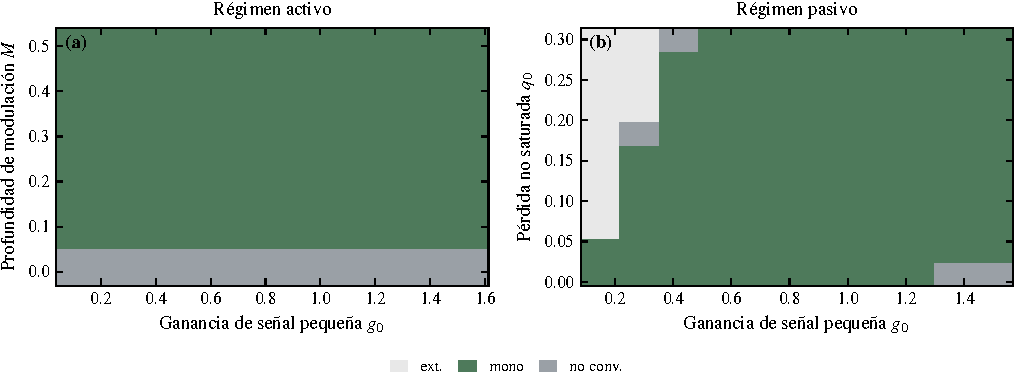
\includegraphics[width=\textwidth]{chapters/images/ch5/fig_val_mapa_regimenes.pdf}
  \caption[Mapa de regímenes del estado estacionario]{Mapa de regímenes del estado estacionario: monopulso, extinción (\emph{ext.})
  y falta de convergencia (\emph{no conv.}) sobre el plano de parámetros del régimen
  activo $(g_0, M)$ y del pasivo $(g_0, q_0)$. El monopulso domina el dominio; las
  regiones no productivas se ciñen a las fronteras.}
  \label{fig:res_val_mapa_regimenes}
\end{figure}

Por último se fija la resolución numérica. La Figura~\ref{fig:res_val_consistencia}
muestra la duración del pulso en función del número de puntos de malla $N$: a partir de
$N=1024$ el valor se estabiliza dentro de una banda del $\pm1\%$ respecto de la malla
más fina, mientras que la energía permanece invariante hasta la precisión de máquina.
La malla de producción, $N=2048$, queda holgadamente dentro de esa banda. Con estas
cuatro comprobaciones (perfil, transitorio, mapa de regímenes y consistencia
numérica) el simulador queda validado como entorno de evaluación, cerrando el primer
objetivo específico y habilitando la lectura del resto del capítulo.

\begin{figure}[htbp]
  \centering
  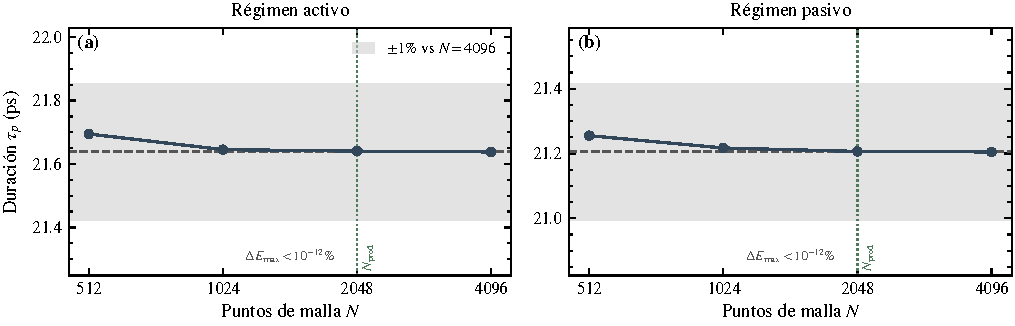
\includegraphics[width=\textwidth]{chapters/images/ch5/fig_val_consistencia.pdf}
  \caption[Consistencia numérica frente a la malla]{Consistencia numérica: duración $\tau_p$ frente al número de puntos de malla
  $N$ en cada régimen. A partir de $N=1024$ el valor cae dentro de la banda del
  $\pm1\%$ respecto de $N=4096$ (sombreado); la energía es invariante hasta $10^{-12}\%$.
  La malla de producción $N_{\mathrm{prod}}=2048$ (línea punteada) está dentro de la
  banda.}
  \label{fig:res_val_consistencia}
\end{figure}

\section{Diseño del contraste y métricas reportadas}
\label{sec:res_diseno}

El estudio enfrenta las tres estrategias, el algoritmo genético (GA), el híbrido con
red neuronal sustituta (NN+GA) y la optimización por enjambre de partículas (PSO),
sobre los dos regímenes de bloqueo de modos, en una matriz de $3\times2$ celdas con
diez repeticiones independientes por celda, es decir, sesenta corridas en total. Cada
corrida parte de una semilla distinta derivada de una secuencia maestra única, lo que
garantiza independencia estadística y reproducibilidad exacta; la verificación de
integridad confirmó las sesenta corridas con sesenta semillas únicas y cobertura
completa de la plataforma de producción. El presupuesto de cómputo se fija en
cuatrocientas evaluaciones del simulador por corrida, idéntico para el GA y el PSO;
el NN+GA consume un calendario propio de setenta evaluaciones reales del simulador
(cuarenta de muestreo inicial por hipercubo latino más treinta de verificación),
sustituyendo el resto por consultas al modelo neuronal. Las condiciones no propias de
cada algoritmo (rangos físicos de las variables de decisión, pesos de la función de
mérito, discretización numérica) se mantienen idénticas para los tres métodos y se
reúnen en la tabla de parámetros de la Sección~\ref{sec:reproducibilidad}.

Sobre cada corrida se reportan cuatro observables. La calidad se resume en el valor
final de la función de mérito, $F^\ast$, y se caracteriza el pulso hallado por su
duración $\tau_p$ y su energía $E$. La eficiencia se cuantifica por el número de
evaluaciones reales del simulador y por las evaluaciones necesarias para alcanzar el
99\% del mejor valor de cada corrida. La robustez se evalúa aparte, en
la Sección~\ref{sec:res_robustez}, mediante la sensibilidad local de $F$ ante
perturbaciones de la solución. Como las réplicas no son normales y las muestras son
pequeñas, los agregados se expresan por su mediana y su rango intercuartílico (IQR),
y las diferencias entre métodos se contrastan con pruebas no paramétricas.

\section{El paisaje de optimización de cada régimen}
\label{sec:res_paisaje}

La variable que vertebra la comparación que sigue no es un algoritmo sino el terreno
sobre el que compiten. Antes de mostrar el desempeño conviene anticipar, desde la física
desarrollada en el Capítulo~\ref{ch:Theoretical background}, que los dos regímenes de
bloqueo de modos plantean paisajes de optimización de naturaleza distinta; esa diferencia
es la lente con la que se leerán todos los resultados posteriores.

% [REV-2026-11-17] matiz: la gaussiana solo vale sin dispersión ni SPM; los óptimos son solitones (ver §5.6)
El régimen activo es el más benigno. Sin dispersión ni no linealidad, la ecuación
maestra con modulación periódica de pérdidas es formalmente análoga a un oscilador
armónico cuántico: admite una familia de soluciones de Hermite--Gauss de las que solo
el modo fundamental es estable, de modo que el estado estacionario es una gaussiana
única y bien definida (Sección~\ref{sec:kuizenga_siegman}) \cite{KuizengaSiegman1970,Keller2022}. Con dispersión anómala y
automodulación de fase, el modulador pasa a estabilizar un solitón, que sigue siendo
un atractor único para cada punto (Sección~\ref{sec:ml_activo_soliton}) \cite{Kaertner2020}. La duración obedece además a una ley de escala
suave, $\tau_p\propto(g/M)^{1/4}$ (ecuación~\eqref{eq:tau_gauss}), en la que la respuesta cambia despacio con los
parámetros (el llamado régimen «duro»). Con solo cuatro variables de decisión
$(g_0,D,\delta,M)$ y un único atractor dominante, el paisaje de la función de mérito es
de baja dimensión, cuasi-unimodal y de gradientes moderados: un terreno regular en el
que la ubicación del óptimo depende poco de la trayectoria seguida para alcanzarlo. Los
resultados matizan esta imagen: en el activo coexisten la familia gaussiana y la
solitónica, y algunas corridas quedan en la primera (Sección~\ref{sec:res_desempeno}).

El régimen pasivo es cualitativamente más difícil. Con el absorbente saturable rápido
ideal, la ecuación maestra adopta la forma de una ecuación de Ginzburg--Landau compleja
generalizada (Sección~\ref{sec:haus_pasivo}), cuya característica distintiva es admitir una variedad de atractores en
lugar de uno solo \cite{Kaertner2020,GreluAkhmediev2012}. Esa multiplicidad es la
expresión matemática de la multiestabilidad física de la cavidad (Sección~\ref{sec:regimenes}) (la coexistencia, para
un mismo vector de parámetros, de onda continua, monopulso, soluciones multipulso y
Q-switching), acompañada de histéresis y de fronteras abruptas entre regímenes. Sobre
cinco variables de decisión $(g_0,D,\delta,q_0,\gamma)$, el paisaje resultante es de mayor
dimensión, no convexo y rugoso, con óptimos locales separados por discontinuidades y
regiones prohibidas. La Figura~\ref{fig:paisaje-regimenes} contrasta esquemáticamente
ambos terrenos. La distinción entre un terreno regular y un terreno accidentado
organiza la lectura de los cuatro bloques de resultados que siguen.

\begin{figure}[t]
    \centering
    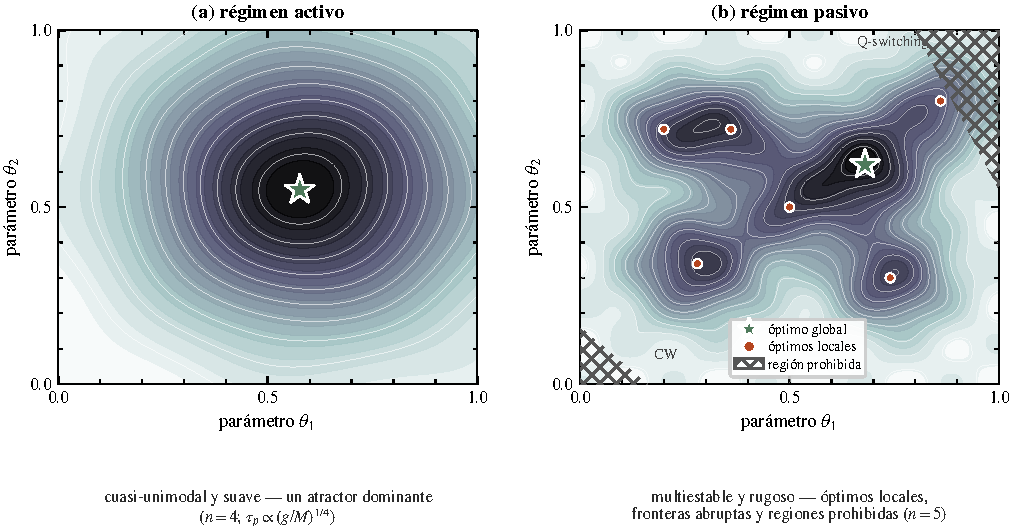
\includegraphics[width=\textwidth]{chapters/images/ch5/fig_paisaje_regimenes.pdf}
    \caption[Paisaje de optimización de cada régimen]{Esquema cualitativo del
    paisaje de la función de mérito en cada régimen, anticipado desde la física del
    Capítulo~\ref{ch:Theoretical background}. \textbf{(a)}~Régimen activo: análogo
    a un oscilador armónico con un único modo de Hermite--Gauss estable, el paisaje
    es de baja dimensión ($n=4$), cuasi-unimodal y de gradientes suaves, un
    atractor dominante y una ley de escala regular $\tau_p\propto(g/M)^{1/4}$,.
    \textbf{(b)}~Régimen pasivo: como ecuación de Ginzburg--Landau compleja con una
    variedad de atractores, el paisaje es de mayor dimensión ($n=5$), no convexo y
    rugoso, con óptimos locales, fronteras abruptas y regiones prohibidas
    (onda continua, \emph{Q\-/switching}). Esta distinción entre un terreno regular
    y uno accidentado es la lente con la que se leen todos los resultados.}
    \label{fig:paisaje-regimenes}
\end{figure}

\section{Desempeño comparado y contraste estadístico}
\label{sec:res_desempeno}

La Tabla~\ref{tab:res_comparativa} reúne los agregados por celda. Las seis celdas
terminan en todas sus repeticiones en un monopulso factible con margen frente a la
inestabilidad de $Q$-switching no negativo, de modo que la comparación se establece
sobre soluciones admisibles y no sobre corridas fallidas.

\begin{table}[htbp]
  \centering\small
  \caption[Desempeño agregado por celda]{Desempeño agregado por celda: mediana [IQR] sobre diez repeticiones.
  $F^\ast$, valor final de la función de mérito; $\tau_p$, duración; $E$, energía;
  \emph{evals}, evaluaciones reales del simulador; \emph{evals$\to$99\%}, mediana de
  evaluaciones hasta el 99\% del mejor valor. En negrita, el mejor
  $F^\ast$ de cada régimen y el presupuesto reducido del NN+GA.}
  \label{tab:res_comparativa}
  \begin{tabular}{llccccc}
    \toprule
    Régimen & Método & $F^\ast$ & $\tau_p$ (ps) & $E$ (nJ) & evals & evals$\to$99\% \\
    \midrule
    \multirow{3}{*}{Activo}
      & GA     & 1.192 [0.197] & 16.3 & 60.8 & 400 & 290 \\
      & NN+GA  & 1.186 [0.172] & 22.2 & 60.8 & \textbf{70} & 19 \\
      & PSO    & \textbf{1.454} [0.052] & 14.2 & 60.2 & 400 & 165 \\
    \midrule
    \multirow{3}{*}{Pasivo}
      & GA     & 2.721 [0.041] & 4.1 & 22.0 & 400 & 222 \\
      & NN+GA  & 2.333 [0.238] & 4.8 & 22.6 & \textbf{70} & 32 \\
      & PSO    & \textbf{2.732} [0.034] & 4.1 & 21.3 & 400 & 288 \\
    \bottomrule
  \end{tabular}
\end{table}

En el régimen activo, el PSO alcanza el mayor valor de mérito, $F^\ast=1.454$, por
encima del GA ($1.192$) y del NN+GA ($1.186$), y lo hace además con la menor
dispersión entre repeticiones (un IQR de $0.052$ frente a $0.197$ del GA) y con la
convergencia más rápida, alcanzando el 99\% de su mejor valor en una
mediana de ciento sesenta y cinco evaluaciones. El GA y el NN+GA quedan prácticamente
empatados en calidad, pero el NN+GA obtiene ese valor con setenta evaluaciones reales
del simulador frente a las cuatrocientas del GA. La Figura~\ref{fig:res_convergencia}
muestra las curvas de mejor-valor-hasta-ahora, donde el marcador señala el fin del
presupuesto real del NN+GA, y la Figura~\ref{fig:res_distribucion} presenta la
distribución de $F^\ast$ por celda, que hace visibles a la vez la ventaja y la menor
dispersión del PSO en este régimen.

\begin{figure}[htbp]
  \centering
  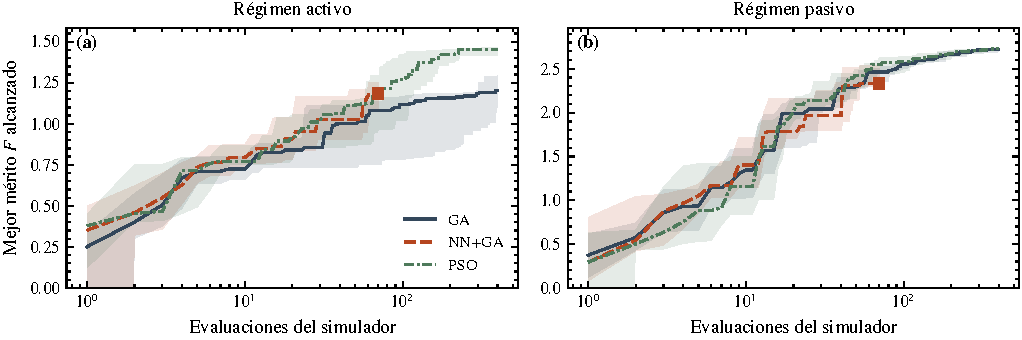
\includegraphics[width=\textwidth]{chapters/images/ch5/fig_convergencia.pdf}
  \caption[Convergencia del mérito por celda]{Convergencia por celda: mediana e IQR del mejor valor de mérito
  alcanzado en función del número de evaluaciones del simulador (eje horizontal
  logarítmico). El marcador sobre las curvas del NN+GA indica el fin de su
  presupuesto real de setenta evaluaciones.}
  \label{fig:res_convergencia}
\end{figure}

\begin{figure}[htbp]
  \centering
  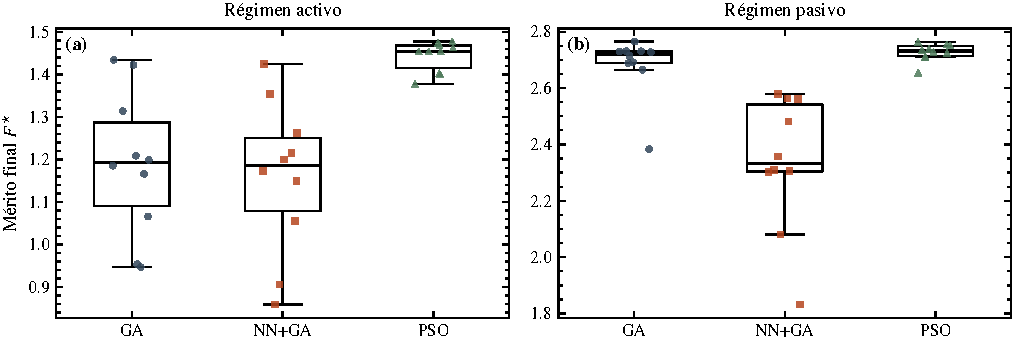
\includegraphics[width=\textwidth]{chapters/images/ch5/fig_distribucion_F.pdf}
  \caption[Distribución del mérito final por celda]{Distribución del valor final de mérito $F^\ast$ por celda (cajas con los
  puntos de las diez repeticiones superpuestos). Se aprecia la ventaja y la menor
  dispersión del PSO en el régimen activo y el empate de las medianas de PSO y GA en
  el pasivo.}
  \label{fig:res_distribucion}
\end{figure}

En el régimen pasivo el panorama cambia. Las medianas de $F^\ast$ del PSO ($2.732$) y
del GA ($2.721$) quedan prácticamente juntas, y ambos convergen a pulsos de la misma
duración ($\tau_p\approx4.1~ps$). El NN+GA, en cambio, se queda por detrás en
calidad ($2.333$) y con mayor dispersión ($\text{IQR}=0.238$). El costo de alcanzar
esa calidad se resume en la Figura~\ref{fig:res_costo}, que reporta las evaluaciones
del simulador necesarias para llegar al $99\%$ del mejor valor de cada corrida, con el
presupuesto de cada método anotado sobre cada barra. Entre las dos búsquedas directas,
el PSO llega antes que el GA en el activo (mediana de $165$ frente a $290$) y algo
después en el pasivo ($288$ frente a $222$); el contraste más visible, el del NN+GA,
se retoma en la Sección~\ref{sec:res_sustituto}.

\begin{figure}[htbp]
  \centering
  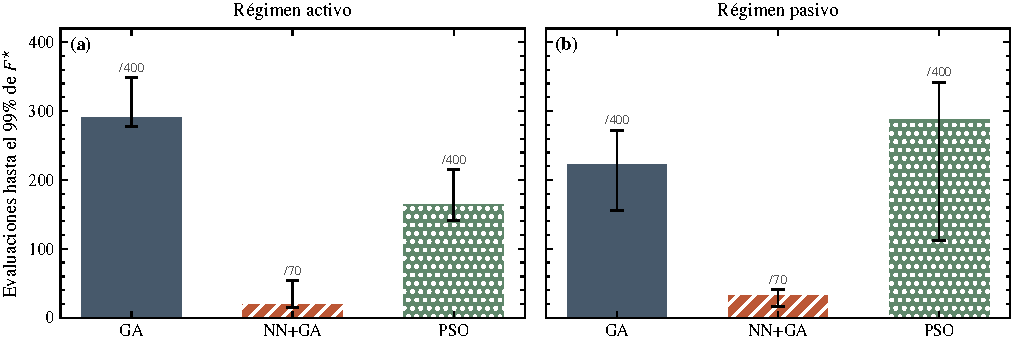
\includegraphics[width=\textwidth]{chapters/images/ch5/fig_costo_convergencia.pdf}
  \caption[Costo de convergencia por celda]{Costo de convergencia: evaluaciones del simulador hasta el $99\%$ del mejor
  valor $F^\star$ por celda (mediana y rango intercuartílico); la anotación sobre cada
  barra indica el presupuesto del método ($/400$ para GA y PSO, $/70$ para NN+GA). El
  NN+GA converge en una fracción de las evaluaciones que gastan las búsquedas directas.}
  \label{fig:res_costo}
\end{figure}

Las diferencias visibles en las Figuras~\ref{fig:res_convergencia}
y~\ref{fig:res_distribucion} se someten a la prueba $U$ de Mann--Whitney bilateral
sobre $F^\ast$, con corrección de Holm para las comparaciones múltiples dentro de
cada régimen. La Tabla~\ref{tab:res_pvalores} resume los $p$ corregidos. Se desprenden
tres resultados. Primero, en el régimen activo el PSO supera de forma significativa
tanto al GA ($p_{\mathrm{Holm}}=0.002$) como al NN+GA ($p_{\mathrm{Holm}}=0.0013$).
Segundo, en el régimen pasivo la diferencia entre PSO y GA no es significativa
($p_{\mathrm{Holm}}=0.27$): las dos búsquedas poblacionales directas quedan
estadísticamente empatadas, aunque ambas superan al sustituto (PSO vs NN+GA,
$p_{\mathrm{Holm}}=0.0006$). Tercero, el NN+GA resulta indistinguible del GA en el
régimen activo ($p_{\mathrm{Holm}}=0.79$) pese a emplear $5{.}7$ veces menos
evaluaciones reales del simulador, un resultado cuya lectura se desarrolla en la
Sección~\ref{sec:res_sustituto}.

\begin{table}[htbp]
  \centering\small
  \caption[Contraste estadístico sobre el mérito]{Contraste estadístico sobre $F^\ast$ ($U$ de Mann--Whitney bilateral,
  $p$ corregido por Holm dentro de cada régimen). En negrita, las diferencias
  significativas al nivel $0.05$.}
  \label{tab:res_pvalores}
  \begin{tabular}{lcc}
    \toprule
    Comparación & $p_{\mathrm{Holm}}$ (activo) & $p_{\mathrm{Holm}}$ (pasivo) \\
    \midrule
    PSO vs GA     & \textbf{0.002}  & 0.27 \\
    PSO vs NN+GA  & \textbf{0.0013} & \textbf{0.0006} \\
    NN+GA vs GA   & 0.79            & \textbf{0.0012} \\
    \bottomrule
  \end{tabular}
\end{table}

La superioridad del PSO en el régimen activo admite una explicación en la naturaleza
del terreno. El PSO guía a cada partícula hacia la mejor posición del enjambre
(\emph{gbest}), lo que produce una convergencia social rápida pero, en contrapartida,
un riesgo elevado de estancamiento prematuro si el paisaje engaña al enjambre hacia un
óptimo local \cite{Kennedy1995}. % [REV-2026-11-17] matiz: el paisaje activo tiene dos familias de soluciones (gaussiana KS y solitónica); ver §5.6
En el régimen activo ese riesgo apenas se materializa para el PSO, aunque el paisaje no
es unimodal: tiene dos familias de soluciones, la gaussiana de Kuizenga--Siegman, con
dispersión y automodulación de fase prácticamente nulas, y la solitónica, de pulsos unas
cuatro veces más cortos y mayor mérito (Sección~\ref{sec:res_fisica}). Ninguna corrida
del PSO terminó en la primera; dos del GA y una del NN+GA, sí. Dentro de la familia
solitónica, la explotación agresiva del PSO se convierte en ventaja y encuentra antes y
con menor varianza los mejores puntos. El GA, cuya
búsqueda es más difusa por diseño (selección, cruce y mutación reparten el presupuesto
entre exploración y explotación), invierte evaluaciones en recorrer un terreno que no
las requiere y llega más tarde y con más dispersión al mismo tipo de solución.

El empate del régimen pasivo confirma la lectura desde el reverso. En un paisaje
multiestable y rugoso, la convergencia social que premia al PSO en el activo se vuelve
un pasivo latente: la misma avidez que acelera la explotación aumenta la probabilidad de
quedar atrapado en uno de los muchos atractores. La exploración más conservadora del GA,
que en el activo era desperdicio, pasa a ser una póliza contra ese estancamiento. Las
dos cinemáticas de búsqueda, ventajosa una y prudente la otra, se compensan sobre un
terreno accidentado y sus desempeños convergen. Dicho de otro modo, la ventaja del PSO
no es una propiedad del método sino del acoplamiento entre el método y el paisaje: existe
cuando el terreno es regular y se disuelve cuando deja de serlo.

% [REV-2026-11-17] lectura física de la ventaja del PSO y control de la esquina (drafts/originalidad/resultados_controles.md, B)
Los parámetros de los óptimos concretan esa lectura. En el régimen activo, $g_0$ queda
en su cota superior o muy cerca de ella en casi todas las corridas de los tres métodos,
así que lo que los distingue son las demás perillas. Entre los treinta óptimos activos,
la duración se correlaciona sobre todo con la automodulación de fase (coeficiente de
Spearman $\rho=-0.69$), después con la profundidad de modulación ($\rho=-0.58$) y con la dispersión ($\rho=+0.40$). El PSO encuentra combinaciones con más automodulación de fase
y más dispersión anómala (medianas de $\delta=1.58\times10^{-4}$~W$^{-1}$ y
$D=-18.1$~ps$^2$, frente a $1.13\times10^{-4}$~W$^{-1}$ y $-13.0$~ps$^2$ del GA), es decir,
un acortamiento solitónico más fuerte (Sección~\ref{sec:res_fisica}). Nueve de sus diez
óptimos tienen además $M$ en su cota superior, frente a ninguno del GA. Esa diferencia,
sin embargo, no explica la ventaja: llevar $M$ a su cota en los óptimos del GA, sin
tocar las demás perillas, deja su mérito igual (mediana de $1.191$ frente a $1.192$). La
ventaja del PSO no está en alcanzar la esquina de la caja, sino en la combinación de
dispersión y no linealidad que encuentra.

Este resultado sitúa en contexto los trabajos que han aplicado el PSO al control de
láseres (el diseño inverso de cavidades por enjambre \cite{Kokhanovskiy2021} o el
ajuste reportado más recientemente \cite{Nsoungui2026}), que documentan su eficacia
sobre problemas concretos pero sin un contraste que aísle el efecto del método.
Precisamente porque el presente estudio mantiene fijos el láser, el espacio de
parámetros y la función de mérito, y varía únicamente el algoritmo, puede afirmar que la
ventaja observada es atribuible a la mecánica de búsqueda y no a las particularidades del
caso, una distinción que la literatura organizada como colección de estudios de caso
aislados no permite establecer \cite{Genty2021,Pineau2021}.

\section{El sustituto neuronal: un ahorro condicionado}
\label{sec:res_sustituto}

El hallazgo central para la hipótesis de ahorro se lee en la Tabla~\ref{tab:res_comparativa}
junto con el contraste de la Tabla~\ref{tab:res_pvalores}: el NN+GA iguala al GA en el
régimen activo ($p_{\mathrm{Holm}}=0.79$) empleando $5{.}7$ veces menos evaluaciones
reales del simulador (setenta frente a cuatrocientas), mientras que en el régimen pasivo
sacrifica calidad de forma significativa ($p_{\mathrm{Holm}}=0.0012$). Una lectura del
propio sustituto ayuda a situar ese comportamiento dispar. La
Figura~\ref{fig:res_surrogate} sigue el error de validación (MSE normalizado) de la red
a lo largo de los ciclos de verificación y reentrenamiento: en el régimen activo el error
desciende de forma marcada hasta el último ciclo, mientras que en el pasivo baja más
despacio y se estanca en un valor más alto. Con el mismo presupuesto de muestras, el
sustituto aprende mejor el paisaje activo que el pasivo, y en el pasivo su error sigue
bajando en el último ciclo: el calendario de setenta evaluaciones se queda corto para
ese régimen.

% [REV-2026-11-17] control C (línea base LHS-70 emparejada; data/runs/controles_v1/C_lhs70)
Que el NN+GA iguale al GA no basta para atribuir el ahorro a la red. El NN+GA gasta sus
setenta evaluaciones en dos partes: cuarenta puntos de hipercubo latino y treinta
verificaciones de los puntos que propone la red. Para separar ambas contribuciones se
construyó, después de la producción, una línea base emparejada con cada corrida: los
mismos cuarenta puntos iniciales, regenerados con la semilla registrada, seguidos de
treinta puntos de un segundo hipercubo latino en lugar de las propuestas de la red. La
Tabla~\ref{tab:res_lhs70} resume el resultado.

\begin{table}[t]
  \centering\small
  \caption[Aporte del sustituto frente a un muestreo del mismo costo]{Mediana del
  mejor mérito tras el muestreo inicial (LHS-40), con treinta puntos aleatorios
  adicionales (LHS-70) y con las treinta verificaciones guiadas por la red (NN+GA),
  sobre las diez corridas de cada régimen. La columna central cuenta en cuántas
  corridas el NN+GA supera, iguala o queda por debajo del LHS-70 emparejado; $p$ es el
  de la prueba de rangos con signo de Wilcoxon.}
  \label{tab:res_lhs70}
  \begin{tabular}{lccccc}
    \hline
    Régimen & LHS-40 & LHS-70 & NN+GA & gana / empata / pierde & $p$ \\
    \hline
    Activo & 1.027 & 1.067 & 1.186 & 5 / 4 / 1 & 0.16 \\
    Pasivo & 1.965 & 2.251 & 2.333 & 4 / 4 / 2 & 0.22 \\
    \hline
  \end{tabular}
\end{table}

Cuando la red acierta, la mejora es grande (entre $+0.07$ y $+0.70$ en mérito), pero en
cuatro de cada diez corridas sus propuestas no superan al mejor punto del muestreo
inicial, y con diez repeticiones su efecto no se distingue del de gastar esas treinta
evaluaciones al azar. Un segundo dato matiza el empate con el GA en el régimen activo:
el LHS-70, sin optimización alguna, tampoco se distingue del GA con cuatrocientas
evaluaciones (mediana de $1.067$ frente a $1.192$, $p=0.16$ con Mann--Whitney), mientras
que en el pasivo el GA lo supera con claridad ($2.721$ frente a $2.251$, $p=0.0003$). El
ahorro del NN+GA en el activo es real en número de evaluaciones, pero dice tanto de lo
benigno que es ese paisaje para un muestreo bien repartido como de la red. Con este
presupuesto y diez repeticiones, el estudio no permite atribuir a la red una ventaja
propia sobre su muestreo inicial.

\begin{figure}[htbp]
  \centering
  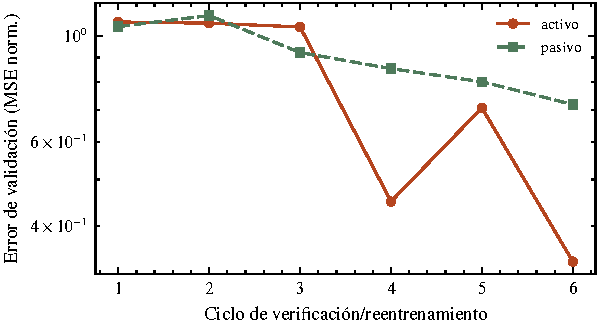
\includegraphics[width=0.7\textwidth]{chapters/images/ch5/fig_surrogate.pdf}
  \caption[Aprendizaje del sustituto neuronal]{Aprendizaje del sustituto: error de validación (MSE normalizado) de la red
  neuronal frente al ciclo de verificación y reentrenamiento, en cada régimen. El error
  cae más y más rápido en el régimen activo que en el pasivo, que se estanca en un valor
  más alto.}
  \label{fig:res_surrogate}
\end{figure}

El mismo paisaje explica ambos comportamientos. La eficacia de un modelo sustituto
depende de que la función objetivo sea aprendible a partir de pocas muestras: un terreno
regular se interpola bien con un puñado de puntos; uno rugoso, no. El sustituto hereda
así la geometría del problema (aprende con más facilidad el paisaje regular del
activo, y tropieza con la variedad de atractores del pasivo), de modo que el ahorro solo
se realiza donde el paisaje lo consiente. Este matiz cualifica la promesa de los métodos
de sustitución tal como la presenta la literatura, donde las redes se emplean para
aproximar la propagación del pulso \cite{Salmela2021} o para predecir directamente la
configuración óptima \cite{Han2024}: el sustituto no reduce el costo de manera
incondicional, sino a cambio de un supuesto de regularidad del paisaje que el régimen
activo satisface y el pasivo no; y aun en el activo, con setenta evaluaciones, su
aporte no se separa del de su propio muestreo. Reconocer esa condición es tan importante como
constatar el ahorro, porque delimita cuándo conviene desplegar la estrategia. La
consecuencia más aguda de esa dificultad en el régimen pasivo se hará visible en la
robustez de su mejor solución (Sección~\ref{sec:res_robustez}).

\section{Forma física de las soluciones halladas}
\label{sec:res_fisica}

Más allá de qué método gana, las propias soluciones admiten una lectura física. La
separación más marcada entre regímenes es que el pasivo produce pulsos aproximadamente
cuatro veces más cortos que el activo (del orden de $4$~ps frente a $14$--$22$~ps) y con
energías menores, en torno a $22$~nJ frente a $60$~nJ. La Figura~\ref{fig:res_tau_energia}
sitúa las mejores soluciones en el plano duración--energía y hace visible esa separación.

\begin{figure}[htbp]
  \centering
  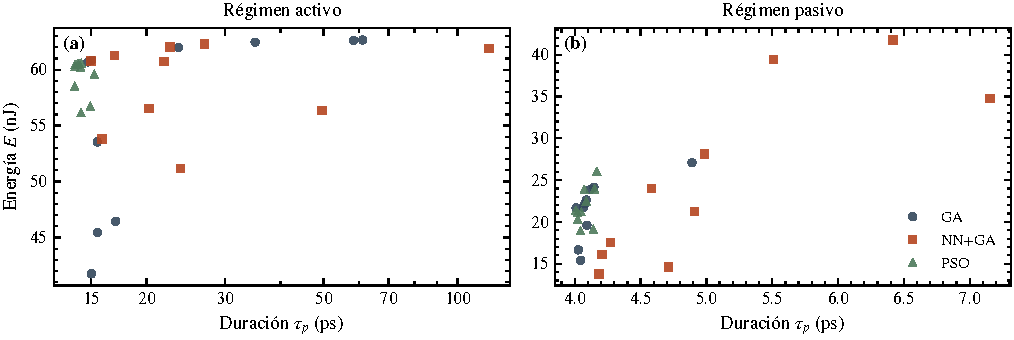
\includegraphics[width=\textwidth]{chapters/images/ch5/fig_tau_energia.pdf}
  \caption[Mejores soluciones en el plano duración--energía]{Mejores soluciones en el plano duración--energía $(\tau_p, E)$ por celda
  (eje de duración logarítmico en el régimen activo). Separación clara entre el
  régimen activo (pulsos largos y energéticos) y el pasivo (pulsos cortos y menos
  energéticos).}
  \label{fig:res_tau_energia}
\end{figure}

% [REV-2026-11-17] corrección: los óptimos activos son solitones sech, no gaussianas (TBP y teorema del área, recalculados)
Las formas de esos pulsos no son incidentales: indican qué física los sostiene. En el
régimen activo, la modulación periódica de pérdidas actúa sobre la envolvente como un
potencial cuasi-armónico cuya solución estable, en ausencia de dispersión y no
linealidad, es la gaussiana de Kuizenga--Siegman (Sección~\ref{sec:kuizenga_siegman}) \cite{KuizengaSiegman1970,Keller2022}.
Los óptimos, sin embargo, casi nunca están en ese límite: veintisiete de los treinta
operan con dispersión anómala y automodulación de fase, en el régimen de bloqueo de modos
activo con formación de solitón (Sección~\ref{sec:ml_activo_soliton}) \cite{Kaertner2020}. Sus pulsos son secantes hiperbólicas
y no gaussianas, con un producto tiempo-ancho de banda de $0.31$ a $0.34$ (el de un pulso sech$^2$ es $0.315$; el de una gaussiana, $0.441$; Sección~\ref{sec:soliton_fundamental}), y su duración
($13.8$ a $15.0$~ps en el mejor punto de cada método) coincide con la que predice el
teorema del área del solitón (ecuación~\eqref{eq:area_soliton}; $13.4$ a $14.7$~ps) y es unas cinco veces menor que la de
Kuizenga--Siegman para los mismos parámetros (ecuación~\eqref{eq:tau_gauss}; $78$ a $82$~ps). Los otros tres óptimos
(dos del GA y uno del NN+GA) tienen dispersión y automodulación de fase prácticamente
nulas y quedan en la gaussiana de Kuizenga--Siegman, con pulsos de $58$ a $118$~ps; son
los de menor mérito de sus celdas.
En el pasivo, el pulso es un solitón disipativo: una secante hiperbólica sostenida no por
la propagación conservativa, sino por un doble balance simultáneo entre dispersión y no
linealidad y entre ganancia y pérdidas (Sección~\ref{sec:soliton_disipativo} y
Figura~\ref{fig:doble-balance}) \cite{GreluAkhmediev2012,Keller2022}. Que la
optimización recupere en cada régimen precisamente la forma que la teoría predice es, por
sí solo, una validación cruzada del entorno de evaluación: el óptimo de calidad coincide
con el atractor físico, no con un artefacto de la búsqueda.

La diferencia de duración se sigue del mecanismo de anclaje. El modulador activo impone
una ventana de baja pérdida de forma fija, sincronizada con el tiempo de ida y vuelta,
que por sí sola solo permite la débil ley de raíz cuarta de Kuizenga--Siegman,
$\tau_p\propto(g/M)^{1/4}$. El acortamiento que consiguen los óptimos activos procede del
balance solitónico entre dispersión y no linealidad, que el modulador se limita a
estabilizar \cite{Kaertner2020}, y aun así queda limitado por esa estabilización. El absorbente saturable del
régimen pasivo, en cambio, ejerce una automodulación de amplitud: el propio pulso satura
la pérdida y abre una ventana de transmisión tanto más estrecha cuanto más corto e intenso
es, en un mecanismo de realimentación positiva que el modulador externo no tiene
(Secciones~\ref{sec:absorbente} y~\ref{sec:haus_pasivo}) \cite{Keller2022}. Esa ventana autoinducida es la razón física por la que el régimen
pasivo alcanza pulsos mucho más breves, y explica por qué la práctica experimental y la
literatura de optimización han privilegiado históricamente este régimen para la generación
de pulsos ultracortos.

La menor energía del pulso pasivo se lee en el mismo marco. Cada régimen alcanza su estado
estacionario sobre un balance distinto, el del solitón estabilizado por el modulador en el activo, con la ganancia apenas por
encima de las pérdidas que imponen el filtrado y la modulación \cite{Kaertner2020}; el
doble balance del solitón disipativo en el pasivo, y la energía resultante es la de ese punto de
operación, no una cantidad que la optimización fije con libertad. % [REV-2026-11-17] corrección: el margen anti-QML nunca estuvo activo (0 de 4338 evaluaciones infactibles)
La frontera de estabilidad frente al $Q$-switching, en cambio, no interviene: el
margen~\eqref{eq:restriccion_qml} fue positivo en todos los óptimos (su mínimo por celda
va de $0.09$ a $0.18$) y no se violó en ninguna de las evaluaciones infactibles de la
matriz. En los dos regímenes, además, $g_0$ quedó en su cota superior o muy cerca de ella,
de modo que la energía de los óptimos es la máxima que sostiene el bombeo admitido en la
caja: unos $60$~nJ en el activo con los tres métodos. La separación en el plano
duración--energía es, en suma, la huella de dos físicas de formación de pulso operando
sobre la misma cavidad de referencia.

Cabe preguntarse, además, si la calidad comparable que alcanzan los métodos corresponde
a soluciones semejantes o a pulsos distintos de mérito parecido. La
Figura~\ref{fig:res_mejor_pulso} superpone el mejor pulso hallado por cada método en cada
régimen: los tres perfiles resultan casi indistinguibles (en el activo, con duraciones de
$13.8$ a $15.0$~ps; en el pasivo, de $4.0$ a $4.2$~ps).

\begin{figure}[htbp]
  \centering
  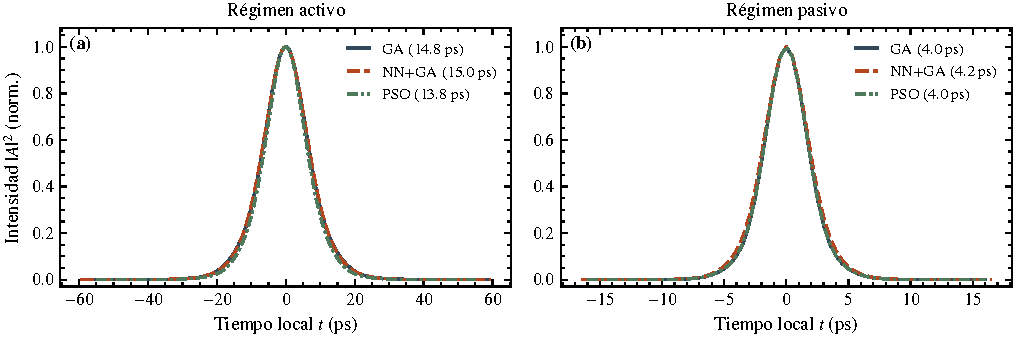
\includegraphics[width=\textwidth]{chapters/images/ch5/fig_mejor_pulso.pdf}
  \caption[Mejor pulso hallado por cada método]{Mejor pulso por método: intensidad $|A|^2$ normalizada de la mejor solución
  de cada algoritmo (duración entre paréntesis). Los perfiles se solapan en ambos
  regímenes, señal de que los métodos convergen a pulsos de la misma forma.}
  \label{fig:res_mejor_pulso}
\end{figure}

Que los tres métodos converjan a la misma forma cuando igualan en mérito confirma, por
último, que el estado estacionario del pulso es un atractor fijado por la física de la
cavidad y no una construcción del optimizador: los algoritmos no moldean el pulso, navegan
hacia el atractor que la dinámica disipativa impone. La función de mérito, al premiar la
brevedad y la energía dentro del régimen factible, empuja además a cada búsqueda hacia el
límite de lo que su física permite (el pulso más corto compatible con la estabilidad), de
modo que el óptimo de calidad se sitúa sobre el borde físico del régimen y no en su
interior. Esta observación anticipa el análisis de robustez: si el óptimo vive contra una
frontera, cabe esperar que resista mal las perturbaciones que lo empujan a cruzarla. Lo
que entonces distingue a un método de otro no es la solución que encuentra, sino la
eficiencia y la fiabilidad con que la alcanza, exactamente el terreno sobre el que la
hipótesis de trabajo situó la comparación.

\section{Robustez local y la frontera de factibilidad}
\label{sec:res_robustez}

La calidad en el óptimo no agota la comparación: importa cuánto se degrada el
desempeño ante pequeñas desviaciones de la solución, inevitables en cualquier
realización física. Para cada celda se toma su mejor corrida y se perturba el punto
óptimo con desplazamientos de $\pm1\%$ del rango de cada variable
($n=16$ perturbaciones), midiendo la caída relativa de $F$; por ello el $F^\ast$ de la
Tabla~\ref{tab:res_sensibilidad} es el de esa mejor corrida y no la mediana reportada
en la Tabla~\ref{tab:res_comparativa}. La tabla recoge la caída mediana y la del peor
caso, y la Figura~\ref{fig:res_robustez} las representa en escala logarítmica con una
línea de referencia en el $100\%$, el umbral a partir del cual la perturbación borra por
completo el mérito de la solución.

\begin{table}[htbp]
  \centering\small
  \caption[Robustez local en torno al óptimo]{Robustez local en torno al óptimo $\mathbf{p}^\ast$ (mejor corrida por
  celda; $n=16$ perturbaciones de $\pm1\%$ del rango). Caída relativa de
  $F$: mediana y peor caso. En negrita, el contraste entre la meseta del PSO y el pico
  frágil del GA en el régimen activo.}
  \label{tab:res_sensibilidad}
  \begin{tabular}{llccc}
    \toprule
    Régimen & Método & $F^\ast$ & Caída mediana & Peor caída \\
    \midrule
    \multirow{3}{*}{Activo}
      & GA     & 1.434 & \textbf{$-601\%$} & $-1484\%$ \\
      & NN+GA  & 1.425 & $-7.3\%$ & $-1306\%$ \\
      & PSO    & 1.477 & \textbf{$-0.7\%$} & $-1215\%$ \\
    \midrule
    \multirow{3}{*}{Pasivo}
      & GA     & 2.765 & $-0.4\%$ & $-733\%$ \\
      & NN+GA  & 2.579 & $+0.6\%$ & $-682\%$ \\
      & PSO    & 2.762 & $-0.4\%$ & $-734\%$ \\
    \bottomrule
  \end{tabular}
\end{table}

\begin{figure}[htbp]
  \centering
  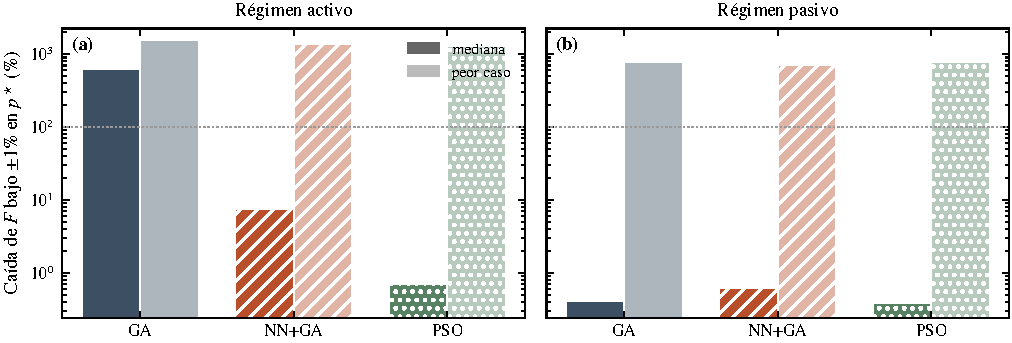
\includegraphics[width=\textwidth]{chapters/images/ch5/fig_robustez.pdf}
  \caption[Robustez local de las soluciones]{Robustez local: caída relativa de $F$ ante perturbaciones de $\pm1\%$ en
  $\mathbf{p}^\ast$ (escala logarítmica), mediana y peor caso por método y régimen. La
  línea punteada marca el $100\%$. En el régimen activo, la mediana del GA supera ese
  umbral (pico frágil) mientras la del PSO queda muy por debajo (meseta); en el pasivo
  las medianas son pequeñas pero el peor caso es severo para los tres.}
  \label{fig:res_robustez}
\end{figure}

La robustez local se revela como una dimensión de comparación que discrimina entre
métodos incluso cuando el valor de mérito los empata. El caso más ilustrativo es el
régimen activo: aunque el mejor punto del GA y el del PSO tienen mérito semejante, su
respuesta a una perturbación difiere por completo. El óptimo del PSO es una meseta (una
caída mediana de apenas $-0.7\%$), mientras que el del GA es un pico frágil cuya
perturbación mediana lo expulsa de la región factible ($-601\%$); el NN+GA queda en una
posición intermedia ($-7.3\%$). Dos soluciones de calidad casi idéntica ocupan posiciones
geométricamente opuestas en el paisaje, y solo el análisis de sensibilidad las separa.
Esta observación tiene una lectura metodológica directa: reportar únicamente el valor de
mérito en el óptimo puede ocultar diferencias de robustez de un orden de magnitud, por lo
que un diseño de comparación honesto debe incorporar la sensibilidad como observable de
pleno derecho, en línea con el énfasis en funciones de mérito compuestas que incluyen
estabilidad \cite{Woodward2016}.

El segundo hecho sobre robustez es común a los tres métodos y a ambos regímenes: el peor
caso es severo en todas las celdas (por debajo de $-1200\%$ en el activo y del orden de
$-700\%$ en el pasivo), aun cuando la mediana sea benigna. En el régimen pasivo los tres
métodos son robustos en mediana (caídas por debajo del $1\%$), y un detalle merece
registro: la caída mediana \emph{positiva} del NN+GA ($+0.6\%$) indica que su mejor punto
no es siquiera un óptimo local, sino un punto en una ladera que un desplazamiento mejora: la firma, en la robustez, del déficit de aprendizaje del sustituto ya visto en la
Sección~\ref{sec:res_sustituto}. La interpretación física del peor caso severo es que
todo óptimo de mérito se apoya contra la frontera de factibilidad en al menos una
dirección. % [REV-2026-11-17] corrección: frontera identificada re-simulando las 16 perturbaciones (control A)
Volver a simular las dieciséis perturbaciones de cada celda permite identificar esa
frontera. En el régimen pasivo es la ruptura del pulso: los puntos perturbados que dejan
de ser factibles pasan a operar en multipulso o no llegan a un estado estacionario, y
ninguno viola el margen frente al $Q$-switching (Cuadro~\ref{tab:regimenes})
\cite{Kaertner2020,GreluAkhmediev2012}.
En el activo es la pérdida del estado estacionario del solitón: los puntos perturbados
infactibles quedan en una dinámica que no se asienta en cincuenta mil vueltas, con una
pulsación periódica de la energía (de unas ochenta y seis vueltas en el peor punto del
NN+GA) o con variaciones irregulares de la duración. Este comportamiento es compatible
con la condición de estabilidad del solitón activo, según la cual el solitón se mantiene
solo si la dispersión anómala domina con suficiente margen a la dispersión de la
ganancia (condición~\eqref{eq:cond_estabilidad_soliton}; deducción en el
Apéndice~\ref{app:soliton_activo}) \cite{Kaertner2020}; confirmarlo exigiría examinar el perfil y el espectro del
campo en esos puntos. El óptimo del PSO es también el más robusto en este sentido:
catorce de sus dieciséis perturbaciones siguen en monopulso, frente a ocho del GA y
nueve del NN+GA. La función de mérito empuja las soluciones
hacia el mejor pulso posible, y el mejor pulso posible se encuentra, por su propia
naturaleza, justo al borde de lo que la cavidad puede sostener: buena parte del entorno
es plana, pero alguna dirección cae por el precipicio. Este comportamiento, esperable en
un sistema disipativo cuyos atractores conviven con regiones prohibidas, aconseja que
cualquier traslado a un montaje real reserve un margen deliberado frente a esas fronteras
en lugar de perseguir el óptimo nominal.

Conviene, por último, dejar constancia de una comprobación que respalda el diseño del
protocolo. Una exploración preliminar de la sensibilidad con solo cuatro perturbaciones
sugería una fragilidad marcada del NN+GA y del PSO en el régimen pasivo; al ampliar la
muestra a dieciséis perturbaciones ese efecto desaparece, revelándose como un artefacto
de muestra pequeña. El episodio ilustra por qué el protocolo exige repeticiones y descarta
conclusiones basadas en corridas aisladas.

\section{Síntesis y límites del estudio}
\label{sec:res_sintesis}

Los resultados admiten una lectura compacta. Sobre la misma función de mérito, las tres
estrategias alcanzan soluciones factibles de calidad comparable, con una excepción
nítida: en el régimen activo el PSO domina en calidad, en dispersión y en velocidad de
convergencia, y su óptimo es además el más robusto. En el régimen pasivo, en cambio, el
PSO y el GA quedan estadísticamente empatados. El NN+GA iguala al GA en el régimen activo con
$5{.}7$ veces menos evaluaciones del simulador y pierde calidad en el pasivo, donde su
mejor punto no es siquiera un óptimo local; el control emparejado muestra, además, que
con este presupuesto su ventaja sobre su propio muestreo inicial no es significativa. La robustez local aparece así como
una tercera dimensión de comparación que discrimina entre métodos incluso cuando el valor
de mérito los empata. Bajo todo ello late un solo factor explicativo: la forma del paisaje
de optimización de cada régimen (más regular en el activo, aunque con dos familias de soluciones, y multiestable y
rugoso en el pasivo) da cuenta a la vez del dominio del PSO, del empate en el pasivo y del
éxito desigual del sustituto.

% [REV-2026-11-17] balance con la hipótesis ajustado a los datos
Estos hallazgos confirman la hipótesis de trabajo solo en parte. Se anticipaba que las
tres estrategias alcanzarían soluciones de calidad comparable pero diferirían de manera
medible en eficiencia y comportamiento de búsqueda, con un método preferible según el
régimen. La segunda parte se cumple; la primera, no del todo: en el activo el PSO supera
en calidad a los otros dos, y en el pasivo el NN+GA queda por debajo. La expectativa de
que el sustituto redujera el costo frente al GA se cumple en número de evaluaciones,
pero el ahorro no puede atribuirse con seguridad a la red, porque el control emparejado
de la Sección~\ref{sec:res_sustituto} no la separa de su muestreo inicial. La conjetura de
que el régimen activo favorecería una convergencia más rápida se cumple para el PSO
($165$ frente a $288$ evaluaciones hasta el $99\%$) y para el NN+GA, pero no para el GA,
que converge antes en el pasivo ($222$ frente a $290$). El único matiz digno de registro es que «método preferible según
el régimen» no se traduce en un ganador uniforme (el PSO domina el activo pero solo
empata en el pasivo), de modo que la recomendación operativa es condicional al régimen de
anclaje y no absoluta. En cuanto a las brechas que motivaron el estudio
(Sección~\ref{sec:aporte}), el trabajo aporta a ambas: frente a la concentración de la
optimización automatizada en el régimen pasivo, muestra que el activo resulta, para esta
familia de metaheurísticas, el régimen \emph{más} tratable (su paisaje favorece la convergencia
rápida del PSO y permite que un muestreo de pocos puntos se acerque al GA, de modo que su
menor presencia en la literatura no obedece a una dificultad intrínseca de optimización); y
frente a los estudios de caso aislados que impiden atribuir las diferencias al algoritmo
\cite{Genty2021,Jiang2022}, el diseño controlado es en sí mismo la contribución.

Estas conclusiones se sostienen dentro de los límites del estudio, que conviene explicitar
para no sobreinterpretarlas. El primero y más importante es la brecha entre la simulación
y el laboratorio: el entorno de evaluación es un modelo idealizado (absorbente rápido
ideal, ausencia de ruido de disparo y de deriva de parámetros, estado estacionario
alcanzado con exactitud) que no reproduce las no idealidades de un montaje experimental,
donde el ruido, la latencia de medición y la deriva térmica modifican tanto el paisaje
como el costo de cada evaluación \cite{Zhao2020,Baumeister2018}. Las conclusiones se
circunscriben, por tanto, al modelo, y su traslado a un oscilador físico es una hipótesis
a verificar, no un corolario. En segundo lugar, el desempeño observado depende de la
cavidad de referencia adoptada, de los rangos de parámetros explorados y de los pesos
fijos de la función de mérito; otras elecciones podrían desplazar los equilibrios, en
particular en la frontera donde PSO y GA empatan.
% [REV-2026-11-17] límites nuevos (cotas activas, pesos re-puntuados, hiperparámetros, penalización)
Dos datos acotan este límite. Por un lado, $g_0$ quedó en su cota superior en casi todas
las corridas, de modo que los óptimos dependen del bombeo máximo admitido en la caja. Por
otro, volver a puntuar los óptimos hallados con pesos de la energía entre $0$ y $2$ no
altera la ventaja del PSO en el activo ($p_{\mathrm{Holm}}$ entre $0.001$ y $0.006$) ni el
empate del pasivo, aunque esta comprobación no sustituye a repetir la optimización con
otros pesos. Los hiperparámetros de los algoritmos, por su parte, se fijaron en valores
habituales y no se ajustaron, y la penalización graduada no se comparó con una plana. En tercer lugar, la robustez se evaluó
como sensibilidad local en torno al óptimo, que no captura la resiliencia global frente a
saltos entre atractores; el peor caso severo advierte precisamente contra leer la mediana
como garantía. Finalmente, el estudio se circunscribe a la familia de optimizadores libres
de gradiente y deja fuera el aprendizaje por refuerzo profundo, cuyo tratamiento de la
multiestabilidad mediante políticas sobre un proceso de decisión \cite{Kokhanovskiy2024}
lo convierte en el horizonte natural de extensión de este trabajo. Ninguna de estas
limitaciones debilita los hallazgos: los delimita, y orienta su lectura hacia lo que el
capítulo de conclusiones recoge como líneas de trabajo futuro.
